\section{Sơ đồ trình tự}
Phần này mô tả trình tự tương tác giữa người dùng, giao diện, máy chủ điều phối và các dịch vụ AI. Các sơ đồ làm rõ cách hệ thống điều phối phiên, xử lý tài liệu và truy vấn RAG theo từng tình huống sử dụng. \cite{lewis2020retrieval}

\subsection{Quy trình quản trị phiên và khởi tạo không gian làm việc}

\begin{figure}[H]
    \centering
    \caption{Sơ đồ trình tự của quy trình quản trị phiên và khởi tạo không gian làm việc}
    \label{fig:sequence-session}
    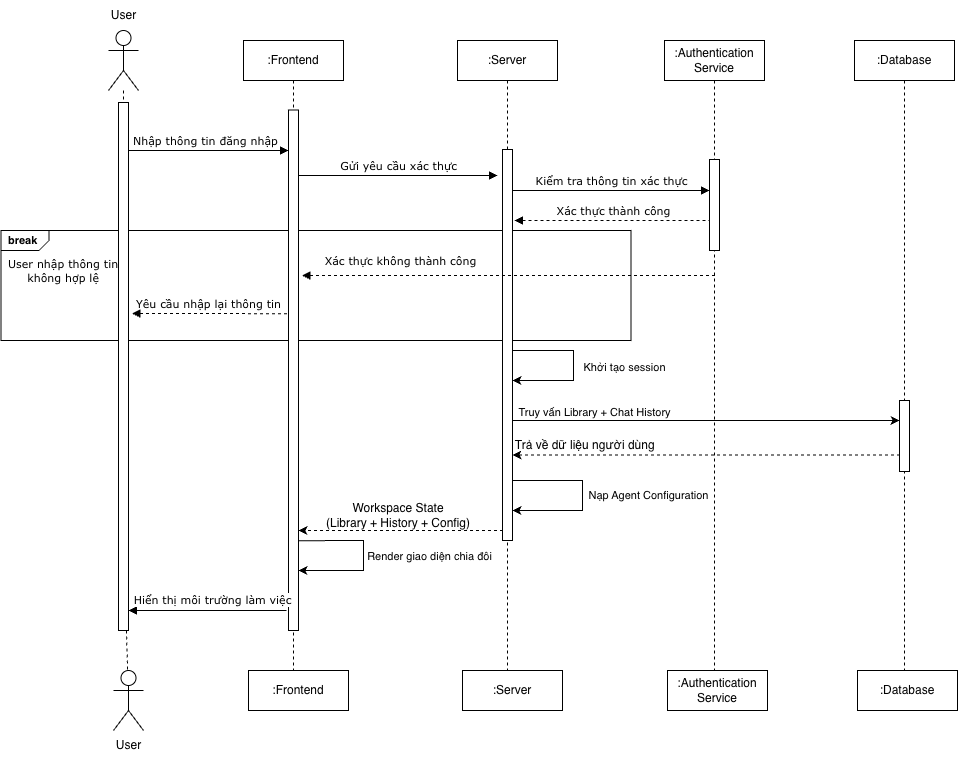
\includegraphics[width=\linewidth]{images/sequence-diagrams/seq-01.png}
\end{figure}

\begin{enumerate}
    \item Giao diện tiếp nhận thông tin xác thực từ người dùng và chuyển tiếp đến máy chủ điều phối.
    \item Máy chủ xác thực và cấp token phiên khi đăng nhập thành công (UC-02).
    \item Máy chủ truy vấn PostgreSQL để lấy danh sách workspace và tài liệu đã nạp.
    \item Cơ sở dữ liệu trả về trạng thái tài liệu và lịch sử hội thoại gần nhất.
    \item Máy chủ gửi toàn bộ trạng thái không gian làm việc về giao diện.
    \item Giao diện dựng màn hình thư viện và danh sách phiên chat.
\end{enumerate}

\subsection{Quy trình quản lý vòng đời và tiền xử lý tài liệu}

\begin{figure}[H]
    \centering
    \caption{Sơ đồ trình tự của quy trình quản lý vòng đời và tiền xử lý tài liệu}
    \label{fig:sequence-preprocess}
    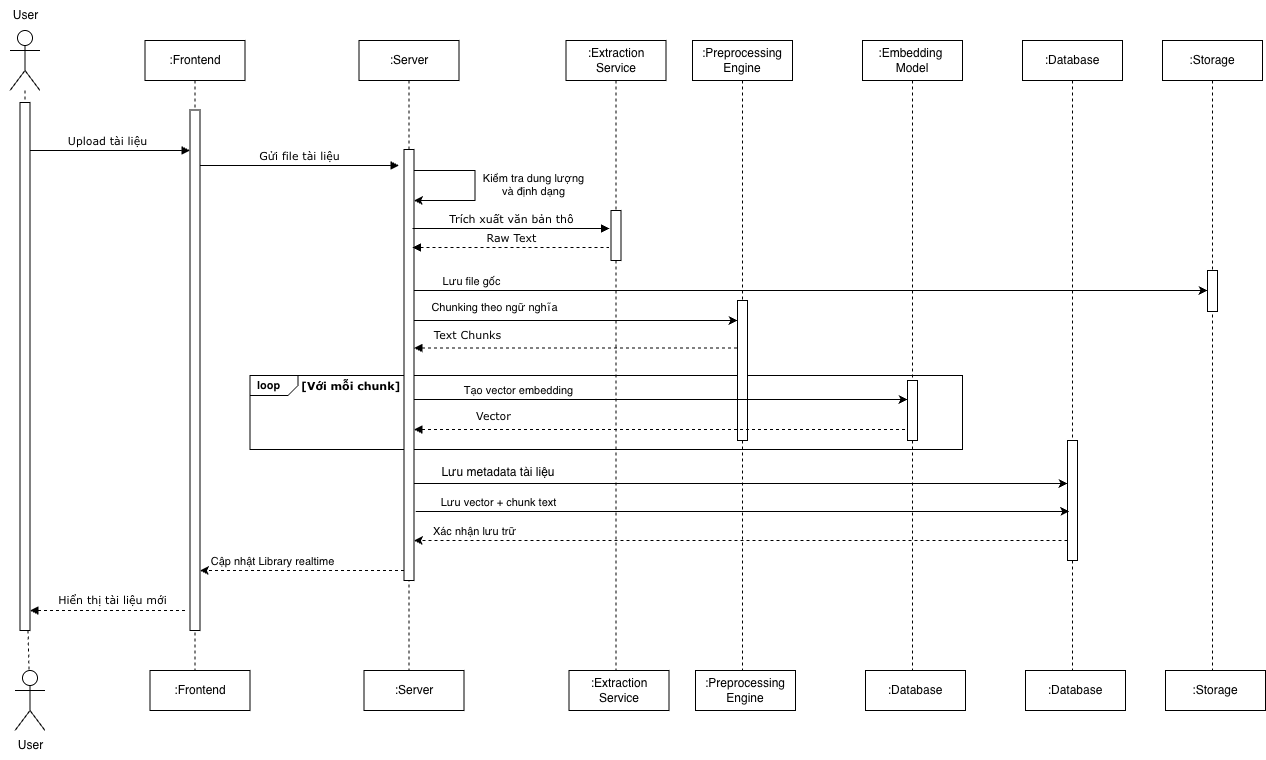
\includegraphics[width=\linewidth]{images/sequence-diagrams/seq-02.png}
\end{figure}

\begin{enumerate}
    \item Người dùng tải tệp tin thông qua giao diện (UC-05).
    \item Máy chủ tiếp nhận tệp, kiểm tra ràng buộc dung lượng/định dạng và trả về ngay mã chấp nhận.
    \item Worker (chạy nền, xem UC-07) gọi dịch vụ trích xuất để bóc tách văn bản và lưu tệp gốc vào kho đối tượng.
    \item Văn bản thô được chuyển đến bộ phân đoạn để chia theo ranh giới cấu trúc và ngữ nghĩa.
    \item Với mỗi phân đoạn, worker gọi dịch vụ nhúng để tạo vector đại diện.
    \item Worker ghi siêu dữ liệu và vector vào PostgreSQL với \texttt{pgvector}.
    \item Giao diện nhận cập nhật trạng thái và làm mới thư viện theo thời gian thực. \cite{reimers2019sentence,pgvector2023}
\end{enumerate}

\subsection{Quy trình hỏi đáp RAG và định tuyến LLM}

\begin{figure}[H]
    \centering
    \caption{Sơ đồ trình tự của quy trình hỏi đáp RAG và định tuyến LLM}
    \label{fig:sequence-rag}
    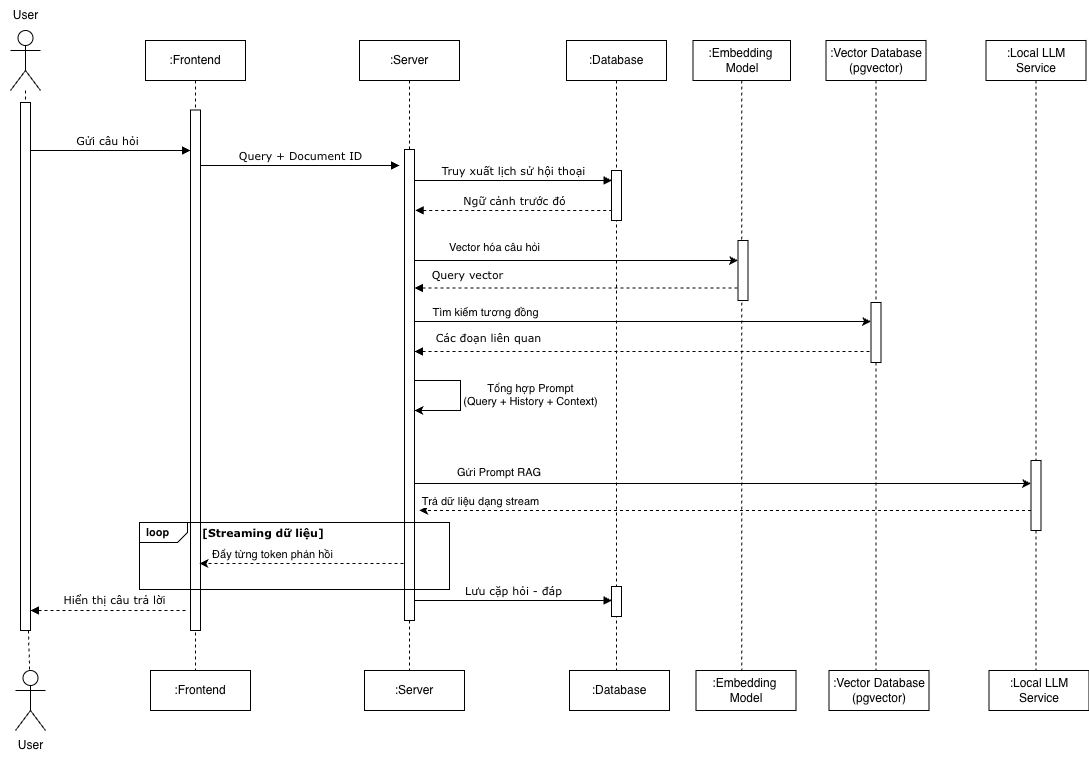
\includegraphics[width=\linewidth]{images/sequence-diagrams/seq-03.png}
\end{figure}

\begin{enumerate}
    \item Người dùng gửi câu hỏi từ khung chat cùng định danh tài liệu mục tiêu (UC-13/UC-14).
    \item Máy chủ truy vấn lịch sử hội thoại của phiên hiện tại để lấy ngữ cảnh trước đó.
    \item Câu hỏi hiện tại được nhúng hóa thành vector truy vấn.
    \item PostgreSQL với \texttt{pgvector} thực hiện tìm kiếm tương đồng và trả về các phân đoạn liên quan nhất.
    \item Máy chủ tổng hợp câu hỏi, ngữ cảnh cứng (nếu có đoạn văn bản được chọn), lịch sử hội thoại và các phân đoạn truy xuất thành một lời nhắc hoàn chỉnh.
    \item Máy chủ gửi lời nhắc đến nhà cung cấp LLM khả dụng đầu tiên trong danh sách ưu tiên của bộ định tuyến (nhãn ``Local LLM Service'' trong sơ đồ đại diện cho bộ định tuyến đa nhà cung cấp thực tế, xem Chương 5).
    \item Máy chủ vừa truyền dữ liệu theo luồng về giao diện, vừa lưu cặp hỏi--đáp mới vào lịch sử phiên. \cite{lewis2020retrieval,gao2023retrieval}
\end{enumerate}
